%preamble
\documentclass[letterpaper]{article}
\synctex=1
\usepackage{graphicx}
\graphicspath{ {images/} }

\usepackage{lipsum}
\usepackage{float}
% \bibliographystyle{IEEEtran}
% \bibliographystyle{ieeetr}

\usepackage{amssymb}

\usepackage{siunitx}

\usepackage{multirow}
% for merging table cells I think

\usepackage{fancyhdr} %header
\fancyhf{}
\fancyhead[R]{Arun Woosaree XXXXXXX}
\renewcommand\headrulewidth{0pt}
\fancyfoot[C]{\thepage}
\renewcommand\footrulewidth{0pt}
\pagestyle{fancy}

% make subsection use letters
\renewcommand{\thesubsection}{\thesection.\alph{subsection}}

%actual document
\begin{document}

% \maketitle %insert titlepage here
\begin{titlepage}
 \begin{center}
  \vspace*{1cm}
  \Huge
  Stat 235
  \vspace{1cm}
  
  Lab 2
  \vspace{1cm}
  
  WOOSAREE, Arun
  \vspace{1cm}
  
  \Huge
  Lab EL12
  \vspace{1cm}
  
  TA: Jessa Marley
  \vspace{1cm}
  
  \today
  \vfill
 \end{center}
\end{titlepage}

\section{Normal Density}

\subsection{}%1a
% Use normal density sheet. Manipulate the graph and describe the changes.
% Describe change as sigma increases in terms of process
% Effect of the change on alloy strength?



As $\sigma$ increases, there is more variation in the tensile strength (makes
sense, since $\sigma^2=V(x)$). This is seen visually as the curve flattening as
a result of the frequency count of the mode being lowered, and the frequency
counts at the more extreme ends being increased. In terms of tensile strength,
an increase in $\sigma$ does not change the mean but it increases the variation
in tensile strength. This does, however mean that less of the alloy produced
will be around the mean tensile strength, and it would increase the fraction of
alloy slabs with unacceptable tensile strength.

\subsection{}%1b
% Use normal density sheet. Manipulate the graph and describe the changes.
% Describe change as mu increases
% Effect of the change on the fraction of unacceptable alloys?

With lower $\mu$ ($\mu=280$ for example), the graph appears left-skewed. This
increases the fraction of unacceptable alloys with $TS < 275$. At $\mu=285$, the
graph appears to be symmetric, and at higher $\mu$ ($\mu=290$ for example), the
graph appears right-skewed. This increases the fraction of unacceptable alloys
with $TS > 295$. Overall, as $\mu$ increases, the tensile strength of the alloys
increase, which causes the fraction  of unacceptable alloys below 275 to
decrease and the fraction above 295 to increase.

% \begin{figure}[H]
%  \centering
%  \includegraphics[width=\textwidth]{x.png}
%  \caption{}
%  \label{}
% \end{figure}

\section{} %2
% #2
% use the normal probablities sheet

\begin{table}[H]
 \centering
 \begin{tabular}{c|c|c|c|}
                      & Parameters                                & Problem                                            & Answer      \\ \hline
  \multirow{2}{*}{a)} & $\mu=285$ and $\sigma=5$                  & Fraction of unacceptable                           & 0.045500264 \\ \cline{2-4}
                      & $\mu=283$ and $\sigma=5$                  & Fraction of unacceptable                           & 0.062996828 \\ \hline
  b)                  & $\mu=285$ and $\sigma=6$                  & Fraction of unacceptable                           & 0.095580705 \\ \hline
  \multirow{2}{*}{c)} & \multirow{2}{*}{$\mu=285$ and $\sigma=5$} & Within 1 std. deviation                            & 0.6827      \\ \cline{3-4}
                      &                                           & Within 2 std. deviations                           & 0.9545      \\ \hline
  \multirow{2}{*}{d)} & \multirow{2}{*}{$\mu=285$ and $\sigma=5$} & Strength exceeded by 95\%                          & 276.78      \\ \cline{3-4}
                      &                                           & Strength exceeded by 99\%                          & 273.37      \\ \hline
  e)                  & $\mu=285$                                 & $\sigma$ so that 1\% have $TS < 275$ or $TS > 295$ & 3.88        \\ \hline
 \end{tabular}
 \caption{How changes in the Mean and Std. Deviation affect the fraction of alloy slabs that do not meet the TS Specifications}
 \label{q2}
\end{table}

\section{Random Number Generator} %3

\subsection{} %generate the random numbers
%3a
% number of unacceptable slabs?
From the randomly generated data, the number of unacceptable slabs is 10.
% consistency with #2a?
$$ {fraction\ unacceptable = \frac{10}{200} = 0.05} $$ 0.05 is reasonably close
to the value 0.045500264, obtained from 2 a) in Table \ref{q2}, so it is
consistent with the theoretical value.

\subsection{}
%3b
%table
% what is the 68-95--99.7 rule?
% are the generated random numbers consitent with this rule?


% \begin{table}[H]
%  \centering
%  \begin{tabular}{|c|c|c|c|}
%   \hline
%   \textbf{k} & \textbf{Within k Std. Deviations of the mean $\mu=285$} & \textbf{Frequency} & \textbf{Relative Frequency} \\ \hline
%   1          & (279.6167494,289.8374972)                               & 129                & 0.645                       \\\hline
%   2          & (274.5063754,294.9478711)                               & 195                & 0.975                       \\ \hline
%   3          & (269.3960015,300.0582451)                               & 199                & 0.995                       \\ \hline
%  \end{tabular}
%  \caption{My caption}
%  \label{my-label}
% \end{table}
%
% \textbf{OR DO WE DO IT THIS WAY}

\begin{table}[H]
 \centering
 \begin{tabular}{|c|c|c|c|}
  \hline
  \textbf{k} & \textbf{Within k Std. Deviations of the mean $\mu=285$} & \textbf{Frequency} & \textbf{Relative Frequency} \\ \hline
  1          & (280, 290)                                              & 130                & 0.65                        \\\hline
  2          & (275, 295)                                              & 190                & 0.95                        \\ \hline
  3          & (270, 300)                                              & 199                & 0.995                       \\ \hline
 \end{tabular}
 \caption{My caption}
 \label{q3}
\end{table}

With relative frequencies of 65\%, 95\%, and 99.5\%, we clearly see that the
data above is consistent with the 68-95-99.7 rule.

\subsection{} % distribution of the standardized values?
%3c
It's a normalized standard distibution. -- \textbf{Do I need a number here??}

k this is my answer for now:
According to the theory, standardizing the values should result in a standard normal distribution.
In practice, we observe a distribution that approximates a standard normal distribution.

\subsection{} % use data analysis -> descriptive statistics tool
%3d
% mean and std deviation fo the standardized values?
% consistency with normal distribution theory?
Using the \textit{Descriptive Statistics Tool}, we find the following from the standardized values:
% $${mean} = -0.0545753437108942$$
% $${std.\ deviation} = 1.02207478598467$$
$$\mu = -0.0546$$
$$\sigma = 1.0221$$
In theory, a standard normal distibution has $\mu=0$, and $\sigma=1$. The values
obtained here are quite close to the expected distribution parameters of a
standard normal distribution, so these values are consistent with the theory.

\section{Changes in Manufacturing Process}%4

\subsection{Summary Statistics} % use data analysis -> descriptive statistics tool
%4a
% consitency with target parameters?
Using the \textit{Desctiptive Statistics Tool, we find that}
$$\mu = 284.6889205$$
$$\sigma = 5.82582628$$
This is consistent with the target parameters $\mu=285$ and $\sigma=5$,
as the values are fairly close, being off by less than a value of 1.

\subsection{Histogram}
%4b
% does it follow a normal distribution?
% does it support the assumption of having a normal distribution
\begin{figure}[H]
 \centering
 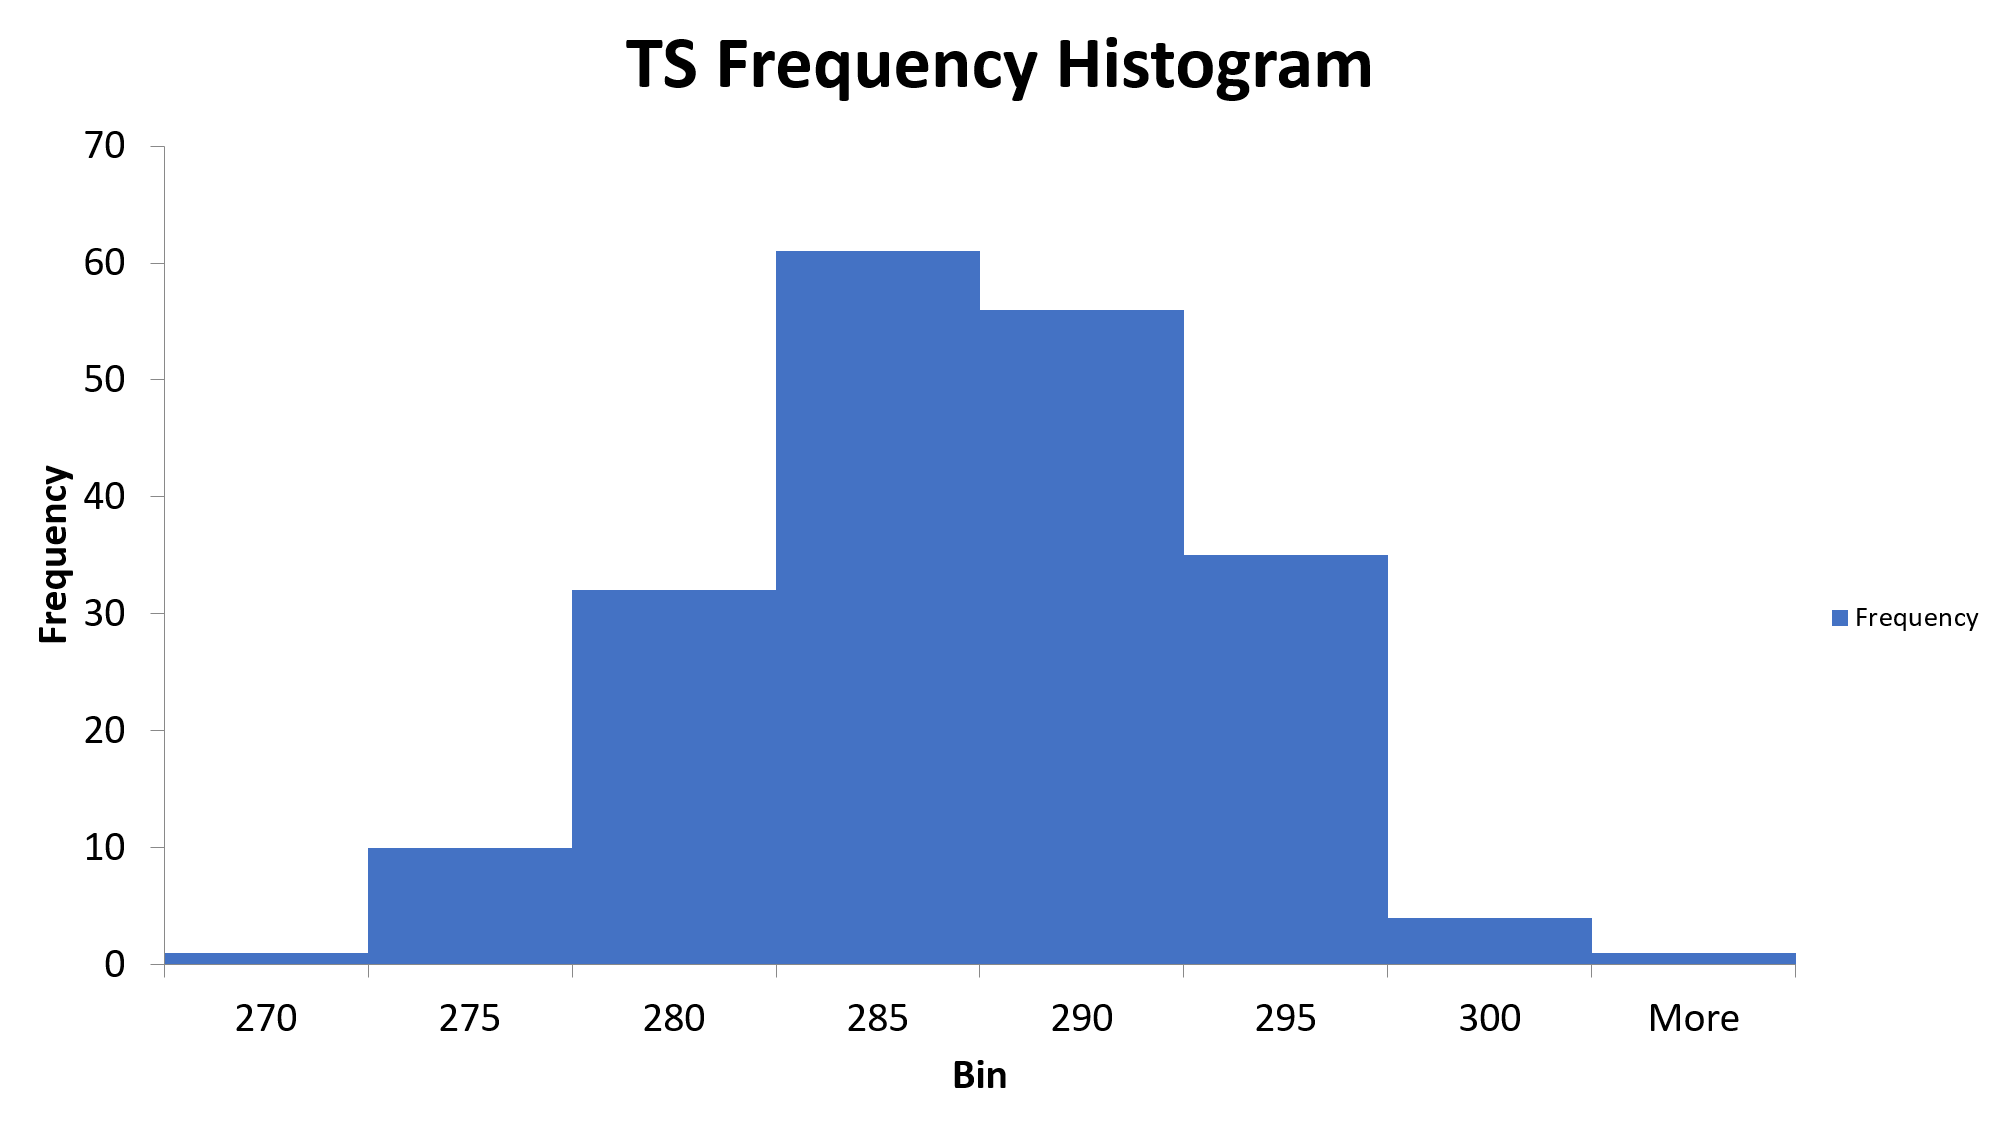
\includegraphics[width=\textwidth]{histogram.png}
 \caption{Relative frequency histogram for 200 observations}
 \label{histogram}
\end{figure}

The histogram above appears to be an approximately symmetric, normal distribution.
There are no glaring indicators which would point to the data not following
a normal distribution.

\subsection{} %use the normal probablities sheet
%4c
% can the manufacturer reach the goal of less than 5% unacceptable?
No. Assuming normality and large sample size, with $\mu = 284.6889205$ and
$\sigma = 5.82582628$, we find that 8.65\% of the slabs produced are
unacceptable, which is above the 5\% limit of unacceptable slabs.

\subsection{} % summarize your findings on TS. Are the changes acceptable?
%4d
The new manufacturing process has slightly lowered the mean tensile strength.
Also, the standard deviation has increased a bit, which may suggest that the new
manufacturing process is slightly less consistent. These changes did not seem to
affect the normality of the distribution in any significant way.

\section{Binomial Probabilities}
%5

\subsection{} % use the binomial probablities sheet.
%5a
% parameters of the distibution?
% binomial probability?
\begin{table}[H]
 \centering
 \begin{tabular}{|l|l|}
  \hline
  n        & 200    \\ \hline
  x        & 15     \\ \hline
  p        & 0.05   \\ \hline
  $P(X>x)$ & 0.0444 \\ \hline
 \end{tabular}
\end{table}

\subsection{} % use the binomial probablities sheet.
%5b
% parameters of the binomial distribution
% (the value of p calculated with the normal probablities sheeet)
% binomial probability?

\begin{table}[H]
 \centering
 \begin{tabular}{|l|l|}
  \hline
  n        & 200               \\ \hline
  x        & 15                \\ \hline
  p        & $1-0.9545=0.0455$ \\ \hline
  $P(X>x)$ & 0.0213            \\ \hline
 \end{tabular}
\end{table}













\end{document}
